\documentclass{article}
\usepackage{fancyhdr}
\usepackage{amsthm}
\usepackage{etoolbox}
\usepackage{verbatim}
\usepackage{enumerate}
\usepackage{amsmath}
\usepackage{algorithmicx}
\usepackage{algorithm}
\usepackage{algpseudocode, algcompatible}
\usepackage{amssymb}
\usepackage{tikz}
	
\pagestyle{fancy}
\title{Chapter 18}
\author{Michelle Bodnar, Andrew Lohr}

\newcounter{curnum}
\setcounter{curnum}{0}

\newtheorem{th1}{Exercise} 
\newcommand{\calH}{\mathcal{H}}
\newcommand{\calX}{\mathcal{X}}
\newcommand{\calA}{\mathcal{A}}
\newcommand{\calY}{\mathcal{Y}}

\begin{document}
\maketitle


\noindent\textbf{Exercise 18.1-1}\\

If we allow $t=0$, then, since we only know that internal nodes have to have at least $t-1$ keys, it may be the case that some internal nodes represent no keys, a bad situation indeed.\\

\noindent\textbf{Exercise 18.1-2}\\

The possible values of $t$ are 2 and 3.  Every non-root node has at least 1 (resp. 2) keys and at most 3 (resp. 5) keys.  The value of $t$ cannot exceed 3 since some nodes have only 2 keys. \\

\noindent\textbf{Exercise 18.1-3}\\

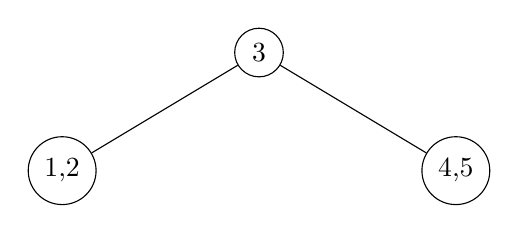
\begin{tikzpicture}[level/.style={sibling distance=50mm/#1}]
\node [circle,draw] (a){3}
  child {
  node [circle,draw] (b) {1,2}
  }
  child {
  node [circle,draw] (i) {4,5}
  };
\end{tikzpicture}

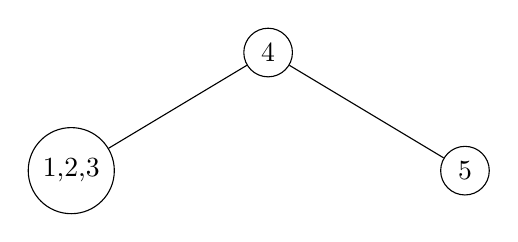
\begin{tikzpicture}[level/.style={sibling distance=50mm/#1}]
\node [circle,draw] (a){4}
  child {
  node [circle,draw] (b) {1,2,3}
  }
  child {
  node [circle,draw] (i) {5}
  };
\end{tikzpicture}

\begin{tikzpicture}[level/.style={sibling distance=50mm/#1}]
\node [circle,draw] (a){4}
  child {
  node [circle,draw] (b) {2}
  child {
  node [circle,draw] (c) {1}
  }
  child {
  node [circle,draw] (d) {3}
  }
  }
  child {
  node [circle,draw] (i) {5}
  };
\end{tikzpicture}

\begin{tikzpicture}[level/.style={sibling distance=50mm/#1}]
\node [circle,draw] (a){2}
  child {
  node [circle,draw] (b) {1}
  }
  child {
  node [circle,draw] (i) {4}
  child{
    node [circle,draw] (c) {3}
}
  child{  node [circle,draw] (d) {5}
}
    };
\end{tikzpicture}

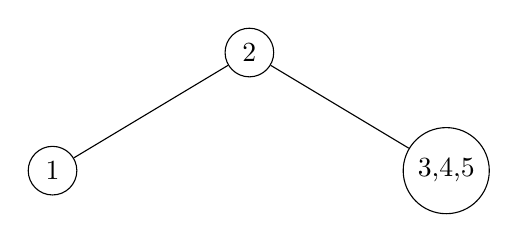
\begin{tikzpicture}[level/.style={sibling distance=50mm/#1}]
\node [circle,draw] (a){2}
  child {
  node [circle,draw] (b) {1}
  }
  child {
  node [circle,draw] (i) {3,4,5}
  };
\end{tikzpicture}

\begin{tikzpicture}[level/.style={sibling distance=50mm/#1}]
\node [circle,draw] (a){2,4}
  child {
  node [circle,draw] (b) {1}
  }
  child {
  node [circle,draw] (i) {3}
  }
    child {
  node [circle,draw] (i) {5}
  };
\end{tikzpicture}

\noindent\textbf{Exercise 18.1-4}\\

The maximum number of nodes is achieved when every node has $2t$ children.  In this case, there are $1 + 2t + (2t)^2 + \ldots + (2t)^h = \frac{1-(2t)^{h+1}}{1-2t}$ nodes.  Since every node has at most $2t-1$ keys, there are at most $(2t)^{h+1} - 1$ keys. \\

\noindent\textbf{Exercise 18.1-5}\\

We would get a t=2 B-tree. It would have one, two, or three keys depending on if it has zero, one, or two red children respectively. Suppose that the left child is red, then it's keys becomes the first one, and that red node's children become the first and second children of the new node. Similarly, if it is the right child that is red, that key becomes the last key listed with the new node, and the red nodes children become the second to last and last children of the new node.\\

\noindent\textbf{Exercise 18.2-1}\\

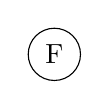
\begin{tikzpicture}[level/.style={sibling distance=50mm/#1}]
\node [circle,draw] (a){F}
  ;
\end{tikzpicture}

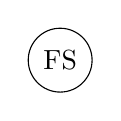
\begin{tikzpicture}[level/.style={sibling distance=50mm/#1}]
\node [circle,draw] (a){FS}
;
\end{tikzpicture}


\begin{tikzpicture}[level/.style={sibling distance=50mm/#1}]
\node [circle,draw] (a){FQS}
;
\end{tikzpicture}

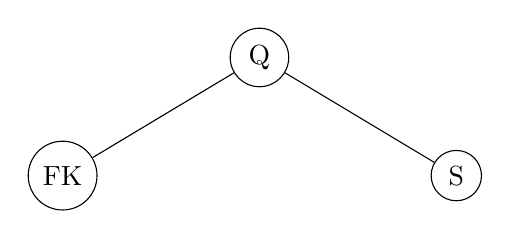
\begin{tikzpicture}[level/.style={sibling distance=50mm/#1}]
\node [circle,draw] (a){Q}
  child {
  node [circle,draw] (b) {FK}
  }
  child {
  node [circle,draw] (i) {S}
  };
\end{tikzpicture}

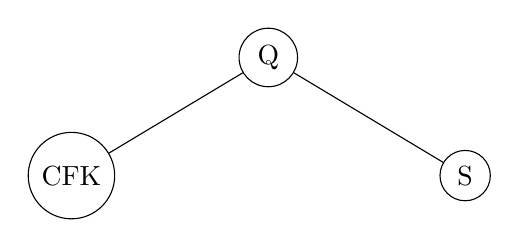
\begin{tikzpicture}[level/.style={sibling distance=50mm/#1}]
\node [circle,draw] (a){Q}
  child {
  node [circle,draw] (b) {CFK}
  }
  child {
  node [circle,draw] (i) {S}
  };
\end{tikzpicture}

\begin{tikzpicture}[level/.style={sibling distance=50mm/#1}]
\node [circle,draw] (a){FQ}
  child {
  node [circle,draw] (b) {C}
  }
  child{
  node[circle,draw] (c){KL}
  }
  child {
  node [circle,draw] (i) {S}
  };
\end{tikzpicture}

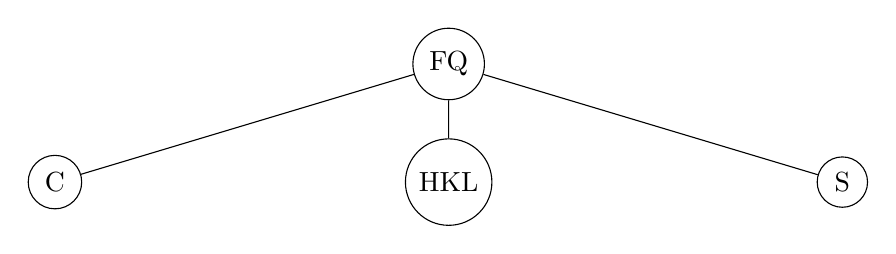
\begin{tikzpicture}[level/.style={sibling distance=50mm/#1}]
\node [circle,draw] (a){FQ}
  child {
  node [circle,draw] (b) {C}
  }
  child{
  node[circle,draw] (c){HKL}
  }
  child {
  node [circle,draw] (i) {S}
  };
\end{tikzpicture}

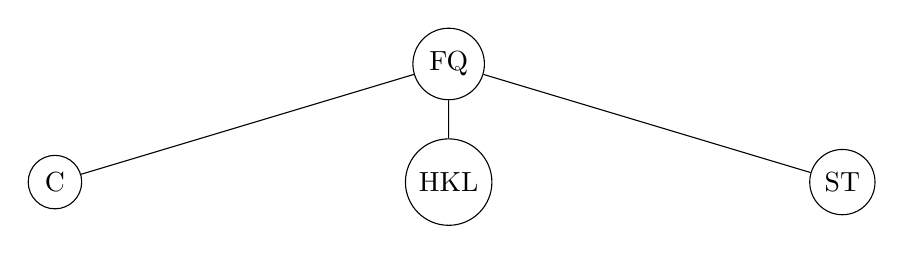
\begin{tikzpicture}[level/.style={sibling distance=50mm/#1}]
\node [circle,draw] (a){FQ}
  child {
  node [circle,draw] (b) {C}
  }
  child{
  node[circle,draw] (c){HKL}
  }
  child {
  node [circle,draw] (i) {ST}
  };
\end{tikzpicture}

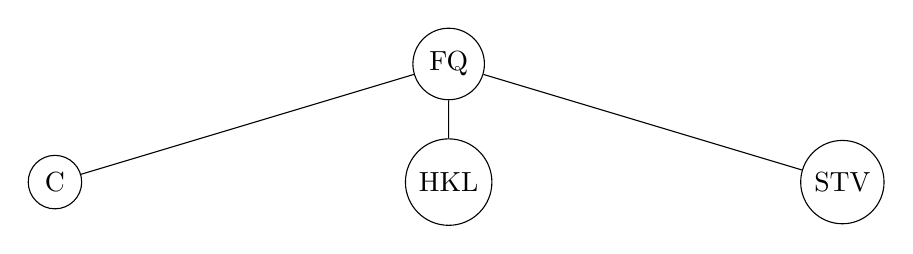
\begin{tikzpicture}[level/.style={sibling distance=50mm/#1}]
\node [circle,draw] (a){FQ}
  child {
  node [circle,draw] (b) {C}
  }
  child{
  node[circle,draw] (c){HKL}
  }
  child {
  node [circle,draw] (i) {STV}
  };
\end{tikzpicture}

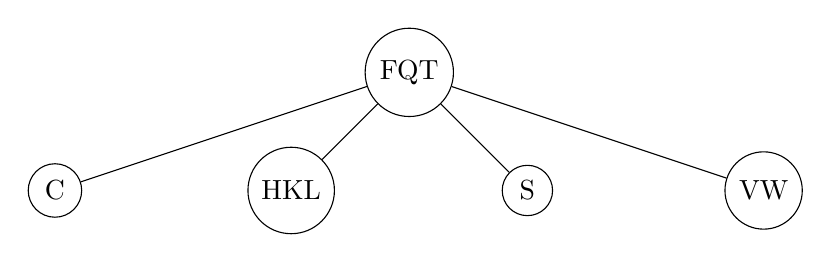
\begin{tikzpicture}[level/.style={sibling distance=30mm/#1}]
\node [circle,draw] (a){FQT}
  child {
  node [circle,draw] (b) {C}
  }
  child{
  node[circle,draw] (c){HKL}
  }
  child {
  node [circle,draw] (i) {S}
  }  child {
  node [circle,draw] (d) {VW}
  };
\end{tikzpicture}

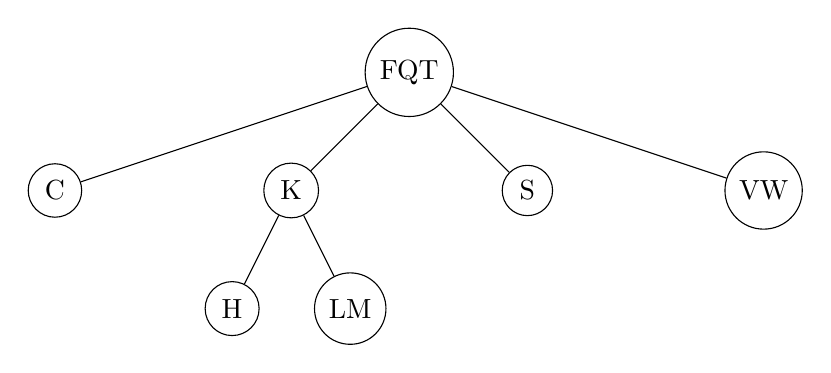
\begin{tikzpicture}[level/.style={sibling distance=30mm/#1}]
\node [circle,draw] (a){FQT}
  child {
  node [circle,draw] (b) {C}
  }
  child{
  node[circle,draw] (c){K}
  child{
  node[circle,draw] (e){H}
  }
  child{
  node[circle,draw] (f){LM}
    }
  }
  child {
  node [circle,draw] (i) {S}
  }  child {
  node [circle,draw] (d) {VW}
  };
\end{tikzpicture}

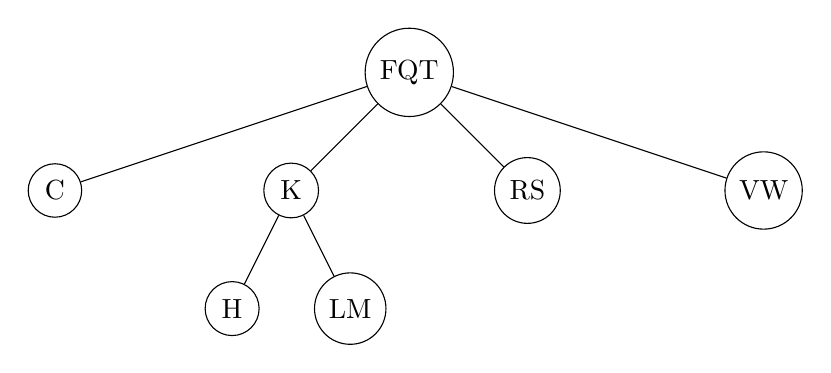
\begin{tikzpicture}[level/.style={sibling distance=30mm/#1}]
\node [circle,draw] (a){FQT}
  child {
  node [circle,draw] (b) {C}
  }
  child{
  node[circle,draw] (c){K}
  child{
  node[circle,draw] (e){H}
  }
  child{
  node[circle,draw] (f){LM}
    }
  }
  child {
  node [circle,draw] (i) {RS}
  }  child {
  node [circle,draw] (d) {VW}
  };
\end{tikzpicture}

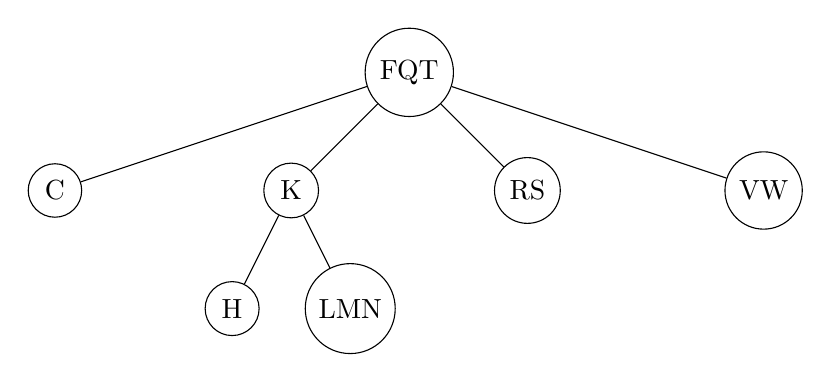
\begin{tikzpicture}[level/.style={sibling distance=30mm/#1}]
\node [circle,draw] (a){FQT}
  child {
  node [circle,draw] (b) {C}
  }
  child{
  node[circle,draw] (c){K}
  child{
  node[circle,draw] (e){H}
  }
  child{
  node[circle,draw] (f){LMN}
    }
  }
  child {
  node [circle,draw] (i) {RS}
  }  child {
  node [circle,draw] (d) {VW}
  };
\end{tikzpicture}

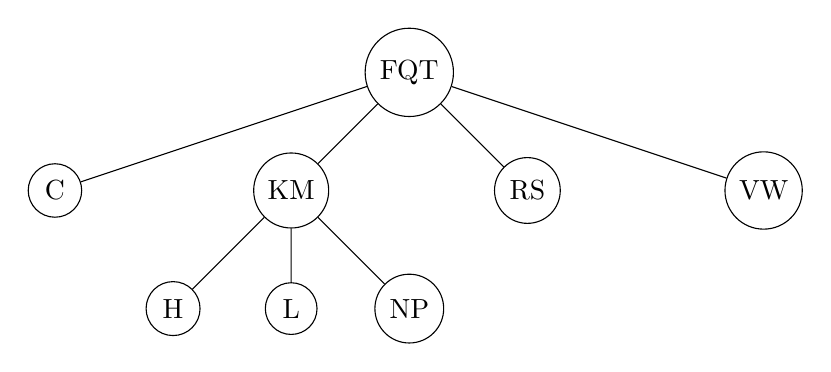
\begin{tikzpicture}[level/.style={sibling distance=30mm/#1}]
\node [circle,draw] (a){FQT}
  child {
  node [circle,draw] (b) {C}
  }
  child{
  node[circle,draw] (c){KM}
  child{
  node[circle,draw] (e){H}
  }
  child{
  node[circle,draw] (f){L}
    }
  child{
  node[circle,draw] (g){NP}
    }
    }
  child {
  node [circle,draw] (i) {RS}
  }  child {
  node [circle,draw] (d) {VW}
  };
\end{tikzpicture}

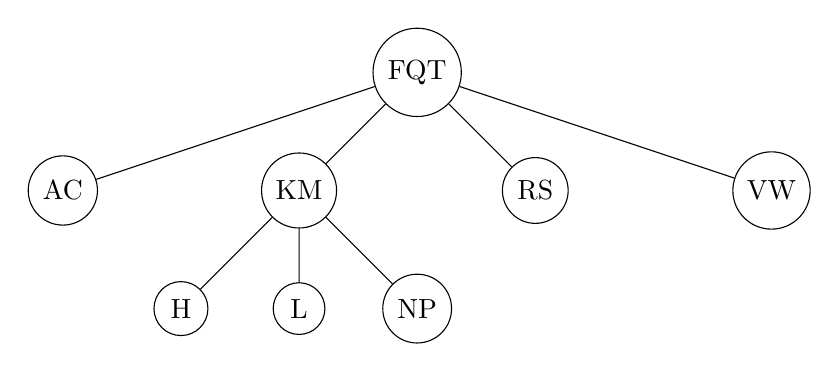
\begin{tikzpicture}[level/.style={sibling distance=30mm/#1}]
\node [circle,draw] (a){FQT}
  child {
  node [circle,draw] (b) {AC}
  }
  child{
  node[circle,draw] (c){KM}
  child{
  node[circle,draw] (e){H}
  }
  child{
  node[circle,draw] (f){L}
    }
  child{
  node[circle,draw] (g){NP}
    }
    }
  child {
  node [circle,draw] (i) {RS}
  }  child {
  node [circle,draw] (d) {VW}
  };
\end{tikzpicture}

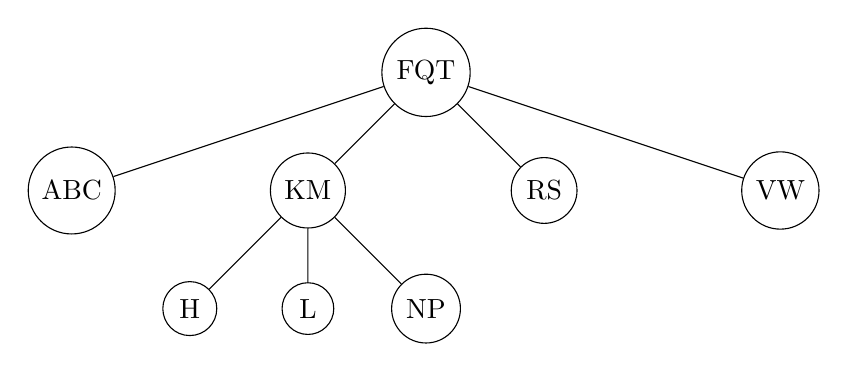
\begin{tikzpicture}[level/.style={sibling distance=30mm/#1}]
\node [circle,draw] (a){FQT}
  child {
  node [circle,draw] (b) {ABC}
  }
  child{
  node[circle,draw] (c){KM}
  child{
  node[circle,draw] (e){H}
  }
  child{
  node[circle,draw] (f){L}
    }
  child{
  node[circle,draw] (g){NP}
    }
    }
  child {
  node [circle,draw] (i) {RS}
  }  child {
  node [circle,draw] (d) {VW}
  };
\end{tikzpicture}

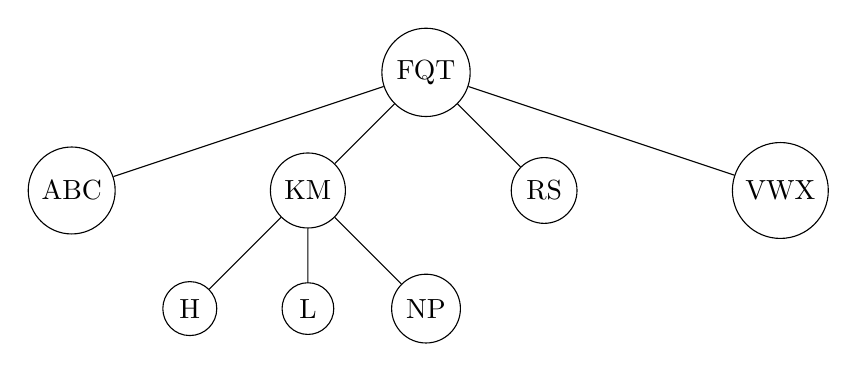
\begin{tikzpicture}[level/.style={sibling distance=30mm/#1}]
\node [circle,draw] (a){FQT}
  child {
  node [circle,draw] (b) {ABC}
  }
  child{
  node[circle,draw] (c){KM}
  child{
  node[circle,draw] (e){H}
  }
  child{
  node[circle,draw] (f){L}
    }
  child{
  node[circle,draw] (g){NP}
    }
    }
  child {
  node [circle,draw] (i) {RS}
  }  child {
  node [circle,draw] (d) {VWX}
  };
\end{tikzpicture}

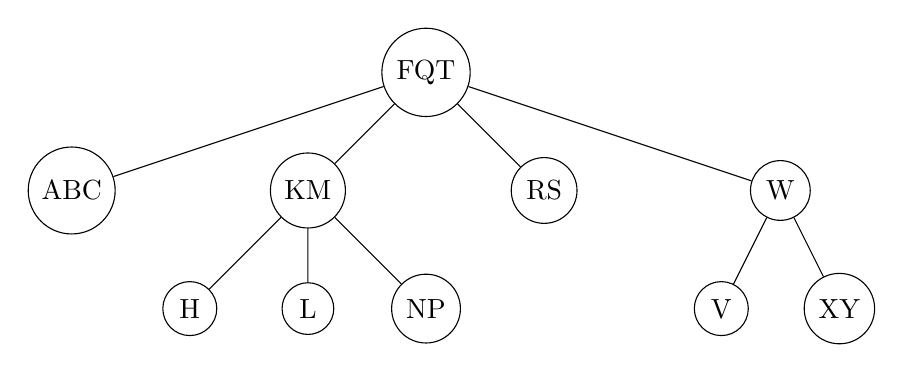
\begin{tikzpicture}[level/.style={sibling distance=30mm/#1}]
\node [circle,draw] (a){FQT}
  child {
  node [circle,draw] (b) {ABC}
  }
  child{
  node[circle,draw] (c){KM}
  child{
  node[circle,draw] (e){H}
  }
  child{
  node[circle,draw] (f){L}
    }
  child{
  node[circle,draw] (g){NP}
    }
    }
  child {
  node [circle,draw] (i) {RS}
  }  child {
  node [circle,draw] (d) {W}
  child{
  node [circle,draw] (h) {V}
  }
  child{
  node [circle,draw] (i) {XY}  
  }
  };
\end{tikzpicture}

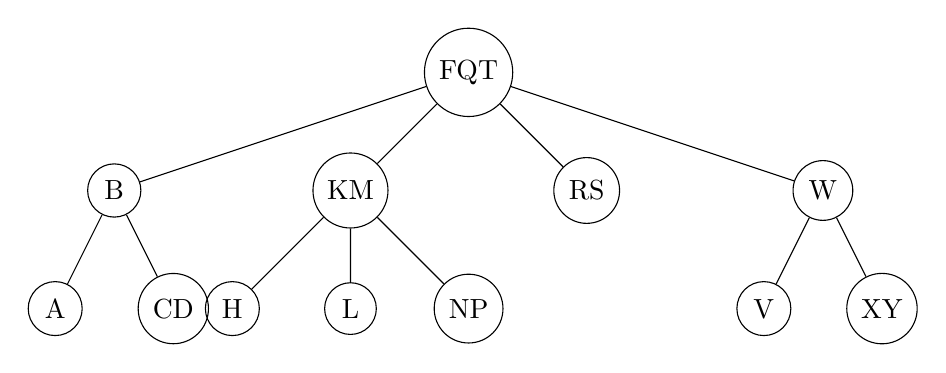
\begin{tikzpicture}[level/.style={sibling distance=30mm/#1}]
\node [circle,draw] (a){FQT}
  child {
  node [circle,draw] (b) {B}
  child{
  node [circle,draw] (j) {A}
    }
  child{
  node [circle,draw] (k) {CD}
  }
  }
  child{
  node[circle,draw] (c){KM}
  child{
  node[circle,draw] (e){H}
  }
  child{
  node[circle,draw] (f){L}
    }
  child{
  node[circle,draw] (g){NP}
    }
    }
  child {
  node [circle,draw] (i) {RS}
  }  child {
  node [circle,draw] (d) {W}
  child{
  node [circle,draw] (h) {V}
  }
  child{
  node [circle,draw] (i) {XY}  
  }
  };
\end{tikzpicture}

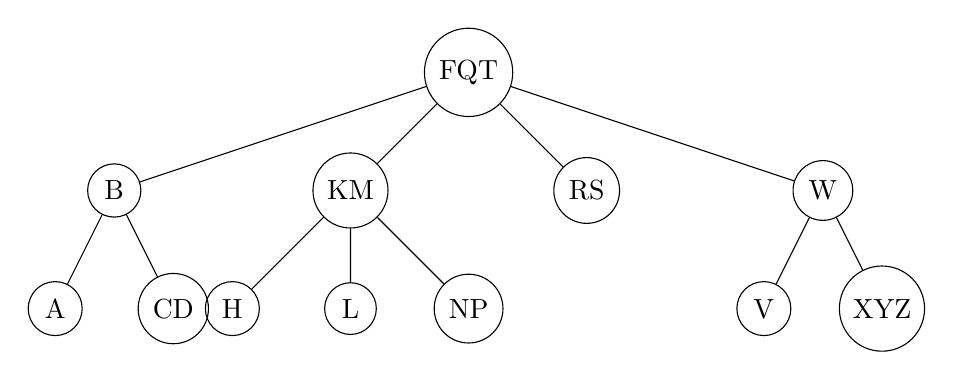
\begin{tikzpicture}[level/.style={sibling distance=30mm/#1}]
\node [circle,draw] (a){FQT}
  child {
  node [circle,draw] (b) {B}
  child{
  node [circle,draw] (j) {A}
    }
  child{
  node [circle,draw] (k) {CD}
  }
  }
  child{
  node[circle,draw] (c){KM}
  child{
  node[circle,draw] (e){H}
  }
  child{
  node[circle,draw] (f){L}
    }
  child{
  node[circle,draw] (g){NP}
    }
    }
  child {
  node [circle,draw] (i) {RS}
  }  child {
  node [circle,draw] (d) {W}
  child{
  node [circle,draw] (h) {V}
  }
  child{
  node [circle,draw] (i) {XYZ}  
  }
  };
\end{tikzpicture}

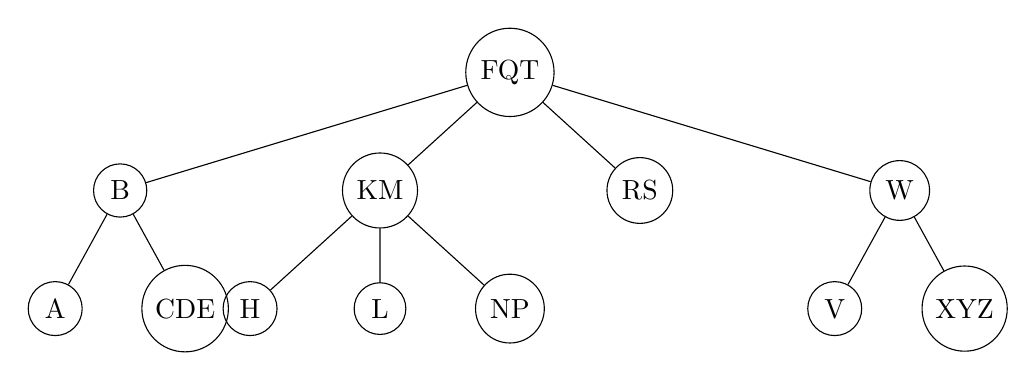
\begin{tikzpicture}[level/.style={sibling distance=33mm/#1}]
\node [circle,draw] (a){FQT}
  child {
  node [circle,draw] (b) {B}
  child{
  node [circle,draw] (j) {A}
    }
  child{
  node [circle,draw] (k) {CDE}
  }
  }
  child{
  node[circle,draw] (c){KM}
  child{
  node[circle,draw] (e){H}
  }
  child{
  node[circle,draw] (f){L}
    }
  child{
  node[circle,draw] (g){NP}
    }
    }
  child {
  node [circle,draw] (i) {RS}
  }  child {
  node [circle,draw] (d) {W}
  child{
  node [circle,draw] (h) {V}
  }
  child{
  node [circle,draw] (i) {XYZ}  
  }
  };
\end{tikzpicture}

\noindent\textbf{Exercise 18.2-2}\\

Lines 1, 2, and 13 of B-TREE-SPLIT-CHILD guarantee that there are no redundant DISK-WRITE operations performed in this part of the algorithm, since each of these lines necessarily makes a change to nodes $z$, $y$, and $x$ respectively.  B-TREE-INSERT makes no calls to DISK-READ or DISK-WRITE.  In B-TREE-INSERT-NONFULL, we only reach line 8 after executing line 7, which modifies $x$, so line 8 isn't redundant.  The only call to DISK-READ occurs at line 12.  Since calls to B-TREE-INSERT-NONFULL are made recursively on successive children, line 12 will never be redundant.  Thus, no redundant read or write operations are ever performed.\\

\noindent\textbf{Exercise 18.2-3}\\

To find the minimum key, just always select the first child until you are on a leaf, then return the first key. To find the predecessor of a given key, fist find it. if it's on a leaf then just return the preceding key. If it's not a leaf, then return the largest element(in an analogous way to finding minimum) of the child that immediately precedes the key just found.\\ 

\noindent\textbf{Exercise 18.2-4}\\

The final tree can have as many as $n-1$ nodes. Unless $n=1$ there cannot ever be $n$ nodes since we only ever insert a key into a non-empty node, so there will always be at least one node with 2 keys.  Next observe that we will never have more than one key in a node which is not a right spine of our B-tree.  This is because every key we insert is larger than all keys stored in the tree, so it will be inserted into the right spine of the tree.  Nodes not in the right spine are a result of splits, and since $t=2$, every split results in child nodes with one key each. The fewest possible number of nodes occurs when every node in the right spine has 3 keys.  In this case, $n=2h + 2^{h+1}-1$ where $h$ is the height of the B-tree, and the number of nodes is $2^{h+1}-1$.  Asymptotically these are the same, so the number of nodes is $\Theta(n)$.\\

\noindent\textbf{Exercise 18.2-5}\\

You would modify the insertion procedure by, in B-TREE-Insert, check if the node is a leaf, and if it is, only split it if there twice as many keys stored as expected. Also, if an element needs to be inserted into a full leaf, we would split the leaf into two separate leaves, each of which doesn't have too many keys stored in it.\\

\noindent\textbf{Exercise 18.2-6}\\

If we use binary search rather than linear search, the CPU time becomes $O(\log_2(t)\log_t(n)) = O(\log_2(n))$ by the change of base formula.\\

\noindent\textbf{Exercise 18.2-7}\\

By Theorem 18.1, we have that the height  of a B-tree on $n$ elements is bounded by $\log_t \frac{n+1}{2}$. The number of page reads needed during a search is at worst the height. Since the cost per page access is now also a function of $t$, the time required for the search is $c(t) = (a+bt)\log_t \frac{n+1}{2}$. To minimize this expression, we'll take a derivative with respect to $t$. $c'(t) = b \log_t\frac{n+1}{2} - (a+bt) \frac{\ln\left(\frac{n+1}{2}\right)}{t \ln(t)^2}$. Then, setting this equal to zero, we have that 
\begin{align*}
b \log_t\frac{n+1}{2} &= (a+bt) \frac{\ln\left(\frac{n+1}{2}\right)}{t \ln(t)^2}\\
b \ln\frac{n+1}{2} &= (a+bt) \frac{\ln\left(\frac{n+1}{2}\right)}{t \ln(t)}\\
t\ln(t) &=(\frac{a}{b} +t)\\
t(\ln(t)-1) &= \frac{a}{b}\\
\end{align*}

For our particular values of $a=5$, and $b=10$, we can solve this equation numerically to get an approximate maxima of 3.18, so selecting t=3 will minimize the worst case cost of a search in the tree.\\



\noindent\textbf{Exercise 18.3-1}\\

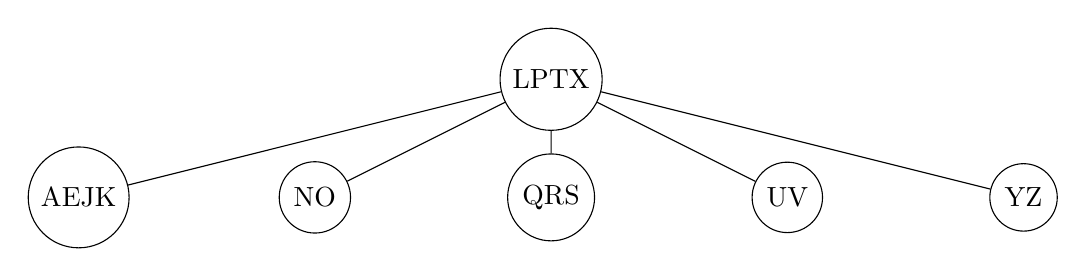
\begin{tikzpicture}[level/.style={sibling distance=30mm/#1}]
\node [circle,draw] (a){LPTX}
  child {
  node [circle,draw] (b) {AEJK}
  }
  child {
  node [circle,draw] (c) {NO}
  }  child {
  node [circle,draw] (d) {QRS}
  }
  child {
  node [circle,draw] (e) {UV}
  }
  child {
  node [circle,draw] (f) {YZ}
  };
\end{tikzpicture}

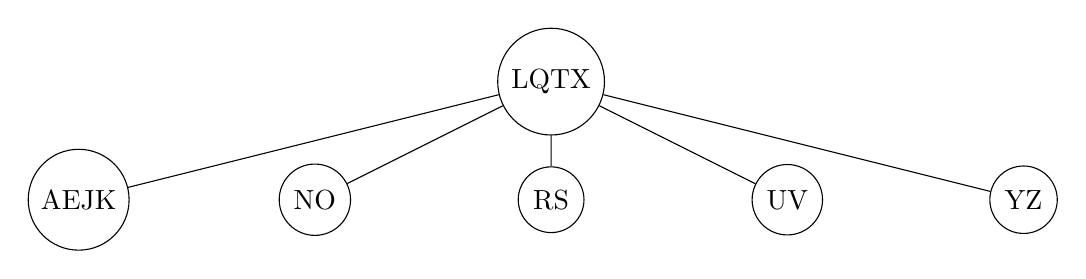
\begin{tikzpicture}[level/.style={sibling distance=30mm/#1}]
\node [circle,draw] (a){LQTX}
  child {
  node [circle,draw] (b) {AEJK}
  }
  child {
  node [circle,draw] (c) {NO}
  }  child {
  node [circle,draw] (d) {RS}
  }
  child {
  node [circle,draw] (e) {UV}
  }
  child {
  node [circle,draw] (f) {YZ}
  };
\end{tikzpicture}

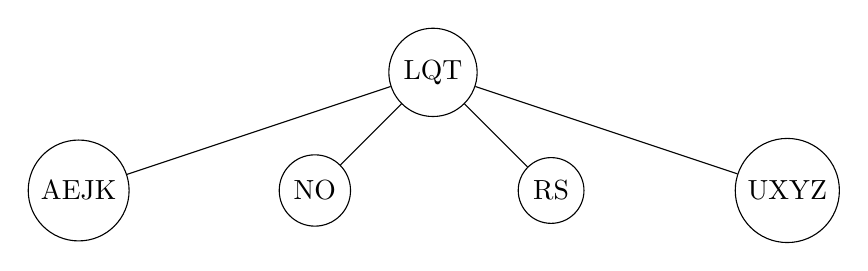
\begin{tikzpicture}[level/.style={sibling distance=30mm/#1}]
\node [circle,draw] (a){LQT}
  child {
  node [circle,draw] (b) {AEJK}
  }
  child {
  node [circle,draw] (c) {NO}
  }  child {
  node [circle,draw] (d) {RS}
  }
  child {
  node [circle,draw] (e) {UXYZ}
  }
;
\end{tikzpicture}\\

\noindent\textbf{Exercise 18.3-2}\\

The algorithm B-TREE-DELETE$(x,k)$ is a recursive procedure which deletes key $k$ from the B-tree rooted at node $x$. The functions PRED$(k,x)$ and SUCC$(k,x)$ return the predecessor and successor of $k$ in the B-tree rooted at $x$ respectively.  The cases where $k$ is the last key in a node have been omitted because the pseudocode is already unwieldy.  For these, we simply use the left sibling as opposed to the right sibling, making the appropriate modifications to the indexing in the for-loops. \\

\begin{algorithm}
\caption{B-TREE-DELETE(x,k)}
\begin{algorithmic}[1]
\IF{$x.leaf$}
	\FOR{$i=1$ to $x.n$}
		\IF{$x.key_i == k$}
			\STATE Delete key $k$ from $x$
			\STATE $x.n = x.n - 1$
			\STATE DISK-WRITE$(x)$
			\STATE Return
		\ENDIF
	\ENDFOR
\ENDIF
\STATE $i = 1$
\WHILE{$x.key_i < k$}
	\STATE $i = i + 1$
\ENDWHILE
\IF{$x.key_i == k$} // If $k$ is in node $x$ at position $i$
	\STATE DISK-READ$(x.c_i)$
	\IF{$x.c_i.n \geq t$}
		\STATE $k' = PRED(k,x.c_i)$
		\STATE $x.key_i = k'$
		\STATE DISK-WRITE$(x)$
		\STATE B-TREE-DELETE$(x.c_i, k')$
		\STATE Return
	\STATE DISK-READ$(x.c_{i+1})$
	\ElsIf{$x.c_{i+1}.n \geq t$}
		\STATE $k' = SUCC(k,x.c_i)$
		\STATE $x.key_i = k'$
		\STATE DISK-WRITE$(x)$
		\STATE B-TREE-DELETE$(x.c_{i+1}, k')$
		\STATE Return
	\Else
		\STATE $y = x.c_i$
		\STATE $z = x.c_{i+1}$
		\STATE $m = y.n$
		\STATE $p = z.n$
		\STATE $y.key_{m+1} = k$
		\FOR{$j=1$ to $p$}
			\STATE $y.key_{m+1+j} = z.key_j$
		\ENDFOR
		\STATE $y.n = m+p+1$
		\FOR{$j=i+1$ to $x.n-1$}
			\STATE $x.c_j = x.c_{j+1}$
		\ENDFOR
		\STATE $x.n = x.n - 1$
		\STATE FREE$(z)$
		\STATE DISK-WRITE$(x)$
		\STATE DISK-WRITE$(y)$
		\STATE DISK-WRITE$(z)$
		\STATE B-TREE-DELETE$(y,k)$
		\STATE Return
	\ENDIF
\ENDIF
\algstore{myalg}
\end{algorithmic}
\end{algorithm}
\begin{algorithm}                     
\begin{algorithmic} [1]                  
\algrestore{myalg}
\STATE DISK-READ$(x.c_i)$
\IF{$x.c_i.n \geq t$}
	\STATE B-TREE-DELETE$(x.c_i,k)$
	\STATE Return
\STATE DISK-READ$(x.c_{i+1})$
\ElsIf{$x.c_{i+1}.n \geq t$}
	\STATE $x.c_i.key_t = x.key_i$
	\STATE $x.c_i.n = x.c_i.n + 1$
	\STATE $x.key_i = x.c_{i+1}.key_1$
	\STATE $x.c_i.c_{t+1} = x.c_{i+1}.c_1$
	\STATE $x.c_i.n = t$
	\STATE $x.c_{i+1}.n = x.c_{i+1}.n - 1$
	\FOR{$j = 1$ to $x.c_{i+1}.n$}
		\STATE $x.c_{i+1}.key_j = x.c_{i+1}.key_{j+1}$
	\ENDFOR
	\STATE DISK-WRITE$(x)$
	\STATE DISK-WRITE$(x.c_i)$
	\STATE DISK-WRITE$(x.c_{i+1})$
	\STATE B-TREE-DELETE$(x.c_i, k)$
\Else
	\STATE $y = x.c_i$
	\STATE $z = x.c_{i+1}$
	\STATE $m = y.n$
	\STATE $p = z.n$
	\STATE $y.key_{m+1} = x.key_i$
	\FOR{$j=1$ to $p$}
		\STATE $y.key_{m+1+j} = z.key_j$
	\ENDFOR
	\STATE $y.n = m+p+1$
	\FOR{$j=i+1$ to $x.n-1$}
		\STATE $x.c_j = x.c_{j+1}$
	\ENDFOR
	\STATE $x.n = x.n - 1$
	\STATE FREE$(z)$
	\STATE DISK-WRITE$(x)$
	\STATE DISK-WRITE$(y)$
	\STATE DISK-WRITE$(z)$
	\STATE B-TREE-DELETE$(y,k)$
	\IF{$x.n == 0$} //This occurs when the root contains no keys
		\STATE Free$(x)$
	\ENDIF
	\STATE Return	
\ENDIF
\end{algorithmic}
\end{algorithm}

\noindent\textbf{Problem 18-1}\\

\begin{enumerate}[a.]
\item
We will have to make a disk access for each stack operation. Since each of these disk operations takes time $\Theta(m)$, the CPU time is $\Theta(mn)$.

\item
Since only every $m$th push starts a new page, the number of disk operations is approximately $n/m$, and the CPU runtime is $\Theta(n)$, since both the contribution from the cost of the disk access and the actual running of the push operations are both $\Theta(n)$.
\item
If we make a sequence of pushes until it just spills over onto the second page, then alternate popping and pulling many times, the asymptotic number of disk accesses and CPU time is of the same order as in part a. This is because when we are doing that alternating of pops and pushes, each one triggers a disk access.
\item
We define the potential of the stack to be the absolute value of the difference between the current size of the stack and the most recently passed multiple of $m$. This potential function means that the initial stack which has size 0, is also a multiple of $m$, so the potential is zero. Also, as we do a stack operation we either increase or decrease the potential by one. For us to have to load a new page from disk and write an old one to disk, we would need to be at least $m$ positions away from the most recently visited multiple of $m$, because we would have had to just cross a page boundary. This cost of loading and storing a page takes (real) cpu time of $\Theta(m)$. However, we just had a drop in the potential function of order $\Theta(m)$. So, the amortized cost of this operation is $O(1)$.
\end{enumerate}
\noindent\textbf{Problem 18-2}\\
\begin{enumerate}[a.]
\item For insertion it will suffice to explain how to update height when we split a node.  Suppose node $x$ is split into nodes $y$ and $z$, and the median of $x$ is merged into node $w$.  The height of $w$ remains unchanged unless $x$ was the root (in which case $w.height = x.height + 1$).  The height of $y$ or $z$ will often change.  We set $y.height = \max_{i} y.c_i.height + 1$ and $z.height = \max_i z.c_i.height + 1$.  Each update takes $O(t)$.  Since a call to B-TREE-INSERT makes at most $h$ splits where $h$ is the height of the tree, the total time it takes to update heights is $O(th)$, preserving the asymptotic running time of insert.  For deletion the situation is even simple.  The only time the height changes is when the root has a single node and it is merged with its subtree nodes, leaving an empty root node to be deleted.  In this case, we update the height of the new node to be the (old) height of the root minus 1. \\

\item Without loss of generality, assume $h' \geq h''$.  We essentially wish to merge $T''$ into $T'$ at a node of height $h''$ using node $x$.  To do this, find the node at depth $h' - h''$ on the right spine of $T'$.   Add $x$ as a key to this node, and $T''$ as the additional child.  If it should happen that the node was already full, perform a split operation.  \\

\item Let $x_i$ be the node encountered after $i$ steps on path $p$.  Let $l_i$ be the index of the largest key stored in $x_i$ which is less than or equal to $k$. We take $k_i' = x_i.key_{l_i}$ and $T_{i-1}'$ to be the tree whose root node consists of the keys in $x_i$ which are less than $x_i.key_{l_i}$, and all of their children.  In general, $T_{i-1}'.height  \geq T_i'.height$. For $S''$, we take a similar approach. They keys will be those in nodes passed on $p$ which are immediately greater than $k$, and the trees will be rooted at a node consisting of the larger keys, with the associated subtrees. When we reach the node which contains $k$, we don't assign a key, but we do assign a tree.\\

\item Let $T_1$ and $T_2$ be empty trees.  Consider the path $p$ from the root of $T$ to $k$.  Suppose we have reached node $x_i$.  We join tree $T_{i-1}'$ to $T_1$, then insert $k_i'$ into $T_1$.  We join $T_{i-1}''$ to $T_2$ and insert $k_i''$ into $T_2$.  Once we have encountered the node which contains $k$ at $x_m.key_k$, join $x_m.c_k$ with $T_1$ and $x_m.c_{k+1}$ with $T_2$.  We will perform at most 2 join operations and 1 insert operation for each level of the tree.  Using the runtime determined in part (b), and the fact that when we join a tree $T'$ to $T_1$ (or $T''$ to $T_2$ respectively) the height difference is $T'.height - T_1.height$.  Since the heights are nondecreasing of successive tree that are joined, we get a telescoping sum of heights.  The first tree has height $h$, where $h$ is the height of $T$, and the last tree has height 0.  Thus, the runtime is $O(2(h + h)) = O(\lg n)$.


\end{enumerate}

\end{document}